\documentclass{beamer}
\title{Detecting Extra-Solar Planets}
\author{Tom Badran}
\date{October 2013 - May 2014}
\begin{document}
\frame{\titlepage}
  \begin{frame}
    \frametitle{Motivations}
    \begin{itemize}
        \item Recent area of research, the first exo-planet was discovered in 1992 orbiting a pulsar (Wolszczan and Frail 1992), and the first orbiting a main-sequence star in 1995 (Mayor and Queloz 1995)
        \item Now up to thousands of planets, many wildly different to our system's planets
        \item They turn out to be very common, finding single and multi planet systems every where, including in binary systems
        \item Aliens! Only just starting to be able to detect possible Earth-like systems
    \end{itemize}
  \end{frame}
  \begin{frame}
    \frametitle{Goals}
    \begin{itemize}
        \item Model planetary transits
        \item Collect and correct images
        \item Perform photometry on these data
        \item Demonstrate planetary detection is possible in the poor seeing conditions of Cardiff
        \item Develop a fully automated processing pipeline for discovering exo-planets
    \end{itemize}
  \end{frame}
  \begin{frame}
    \frametitle{Transit Method}
    \begin{center}
    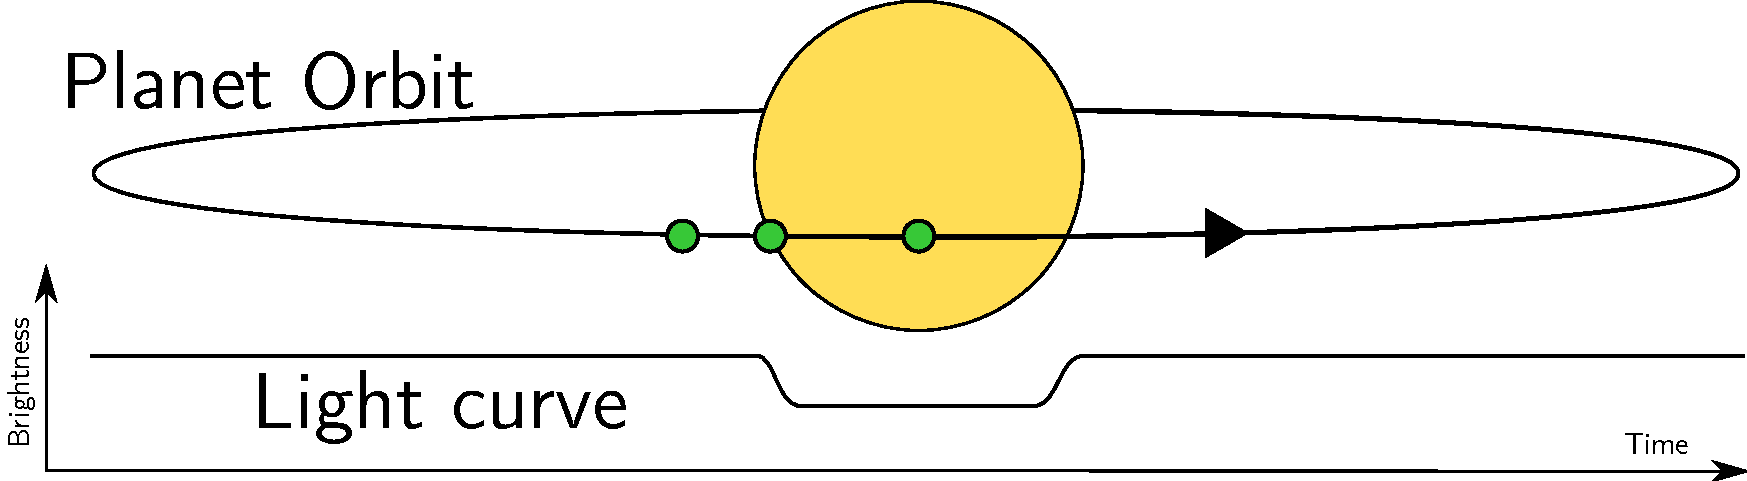
\includegraphics[width=0.8\textwidth]{images/planetary_transit.pdf}
    \end{center}
    As the planet passes between the observer and the star, a portion of the light is blocked, and so a small drop in the apparent brightness of the star is observable.

    Typically these changes are of the order of sub milli-magnitudes to around 20 milli-magnitudes $\Rightarrow$ Hard to detect!
  \end{frame}
  \begin{frame}
    \frametitle{Transit Method}
    Advantages:
    \begin{itemize}
        \item Optical wavelengths
        \item No need for specialist equipment or space telescopes, just need a camera and a clear sky
        \item Determines planet size
    \end{itemize}
    Disadvantages:
    \begin{itemize}
        \item Limited range of inclinations
        \item Poor for stars off the main sequence
        \item Works best for large planets near star (not Earth like)
    \end{itemize}
  \end{frame}
  \begin{frame}
    \frametitle{Modeling}
    \framesubtitle{1st Order - Uniform Disk}
    Model the planet as a solid disk that blocks light completely, and model the star as a solid disk emitting light uniformly.
    \begin{itemize}
        \item No obscuring - 100\% of brightness detected
        \item Fully obscuring - Percentage dip gives radius of the planet
        \item Partially obscured -
    \end{itemize}
    \small
    \begin{align*}
    A &= \kappa_1 + \kappa_2 - \kappa_3 \\
    \kappa_1 &= r_p^2\cos^{-1}\left(\frac{d^2 + r_p^2 - r_*^2}{2dr_p}\right)\\
    \kappa_2 &= r_*^2\cos^{-1}\left(\frac{d^2 + r_*^2 - r_p^2}{2dr_*}\right)\\
        \kappa_3 &= \frac{1}{2}\sqrt{(-d + r_p + r_*)(d + r_p - r_*)(d - r_p + r_*)(d + r_p + r_*)}
    \end{align*}
  \end{frame}
  \begin{frame}
  \frametitle{Modeling}
    \framesubtitle{1st Order - Uniform Disk}
    \begin{center}
    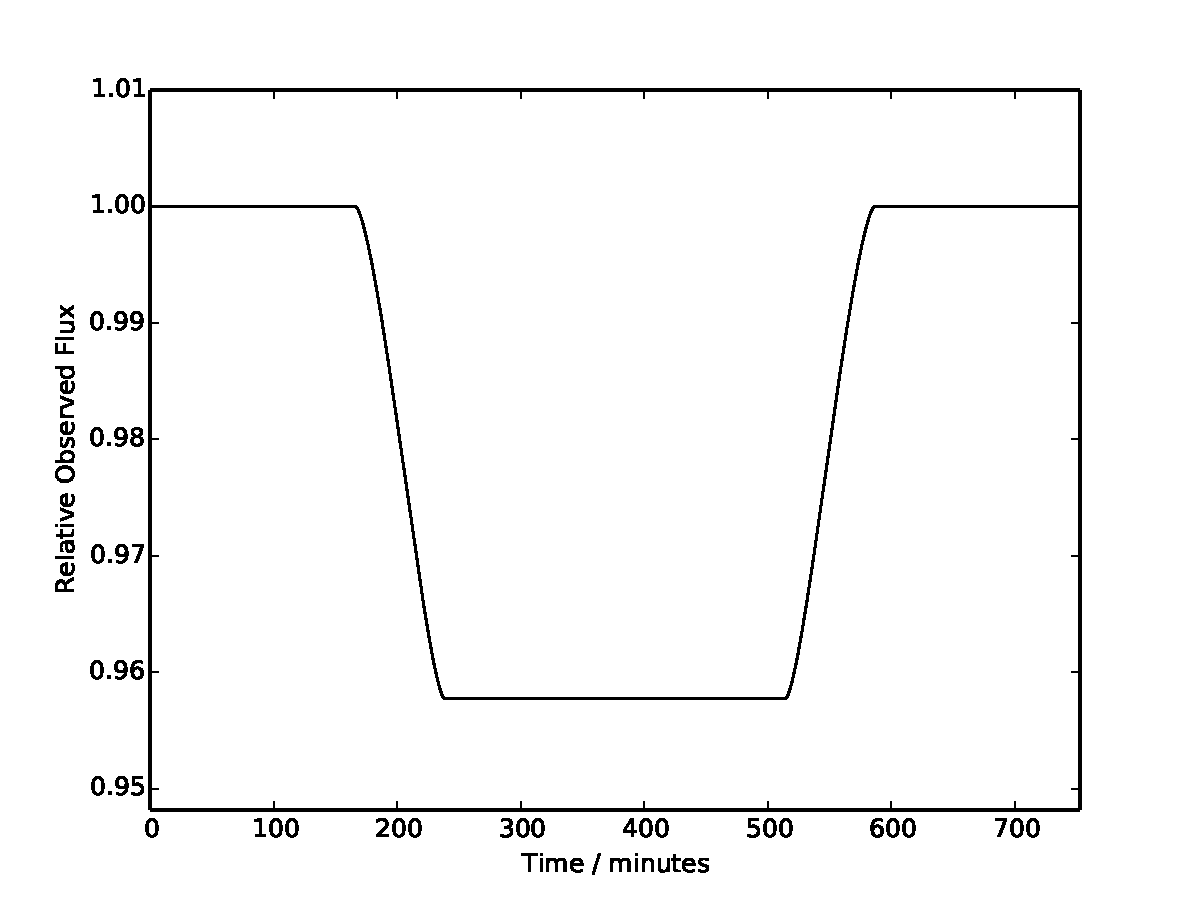
\includegraphics[width=0.9\textwidth]{images/uniform_disk_model.pdf}
    \end{center}
  \end{frame}
  \begin{frame}
  \frametitle{Modeling}
    \framesubtitle{2nd Order - Limb Darkening}
    Planet as solid disk is not bad approximation, atmospheric affects generally fall well into the noise (although some studies have determined properties).
    Star however does not emit uniformly, and is brighter in the center than the towards the edges.
    \begin{center}
    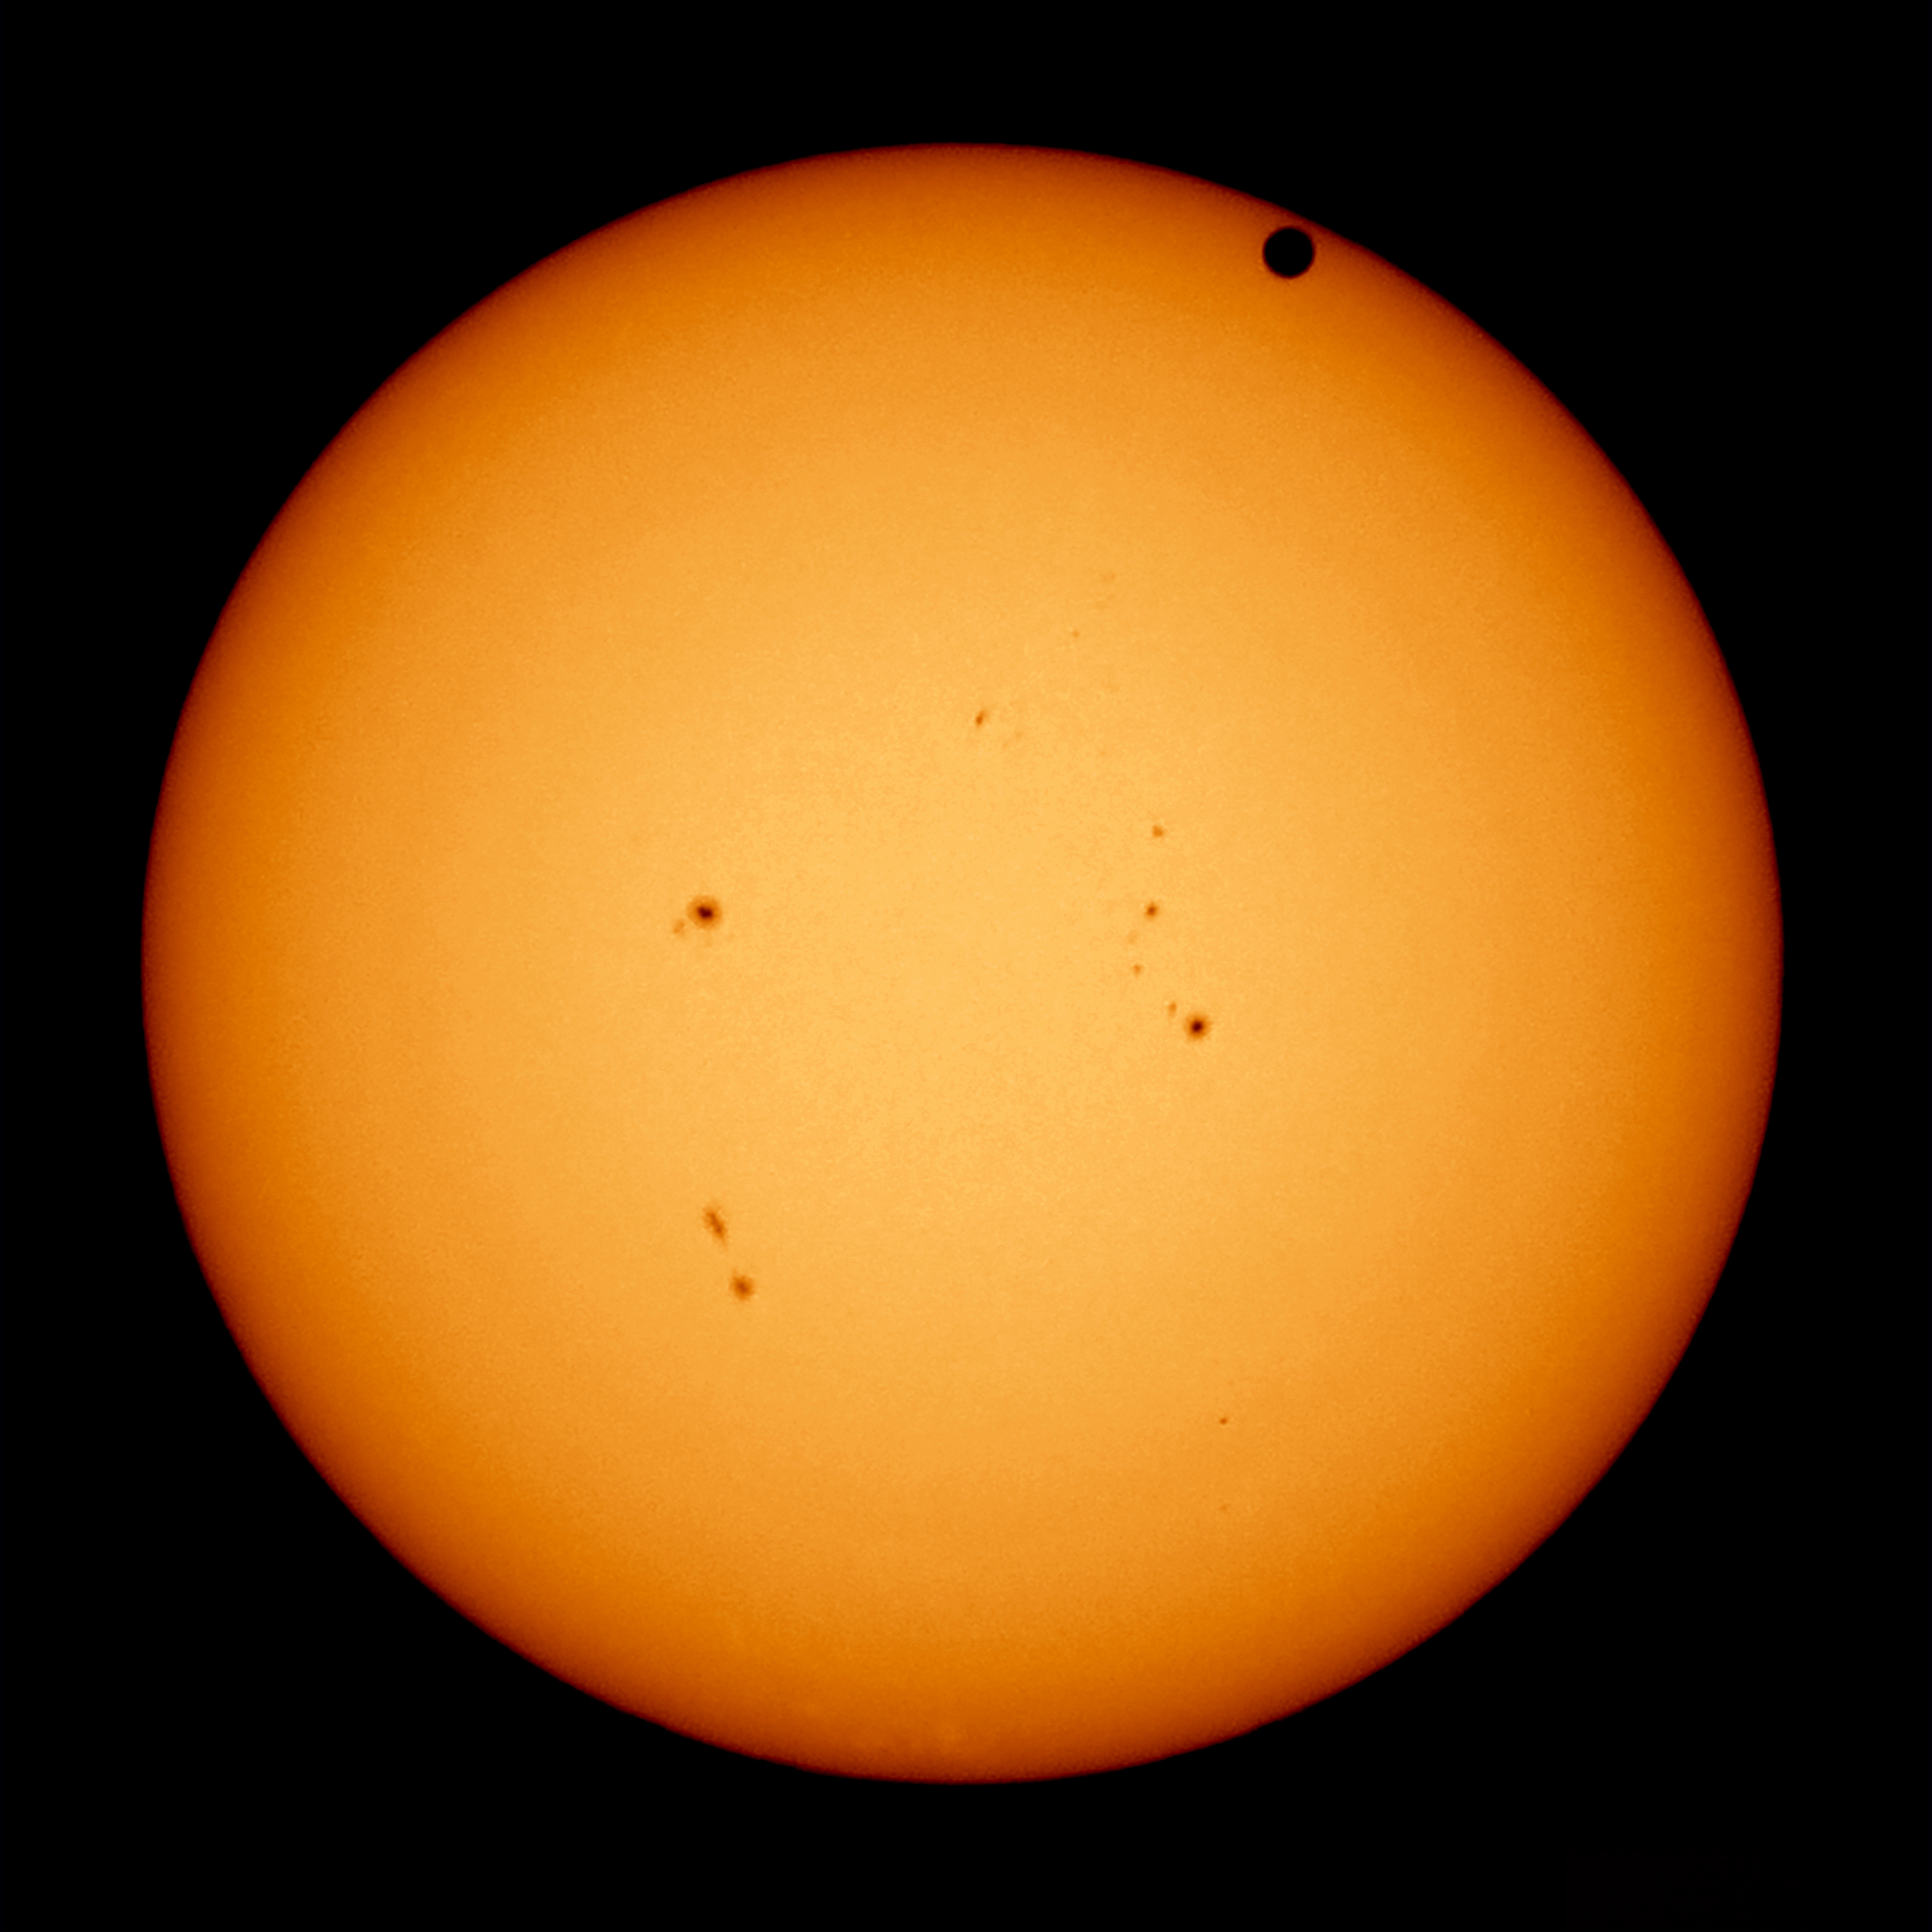
\includegraphics[width=0.4\textwidth]{images/venus_transit.jpg}
    \end{center}
  \end{frame}
  \begin{frame}
  \frametitle{Modeling}
    \framesubtitle{2nd Order - Limb Darkening}
    Modeled as a quadratic function to describe the limb darkening (Mandel and Agol 2002)
    \begin{center}
    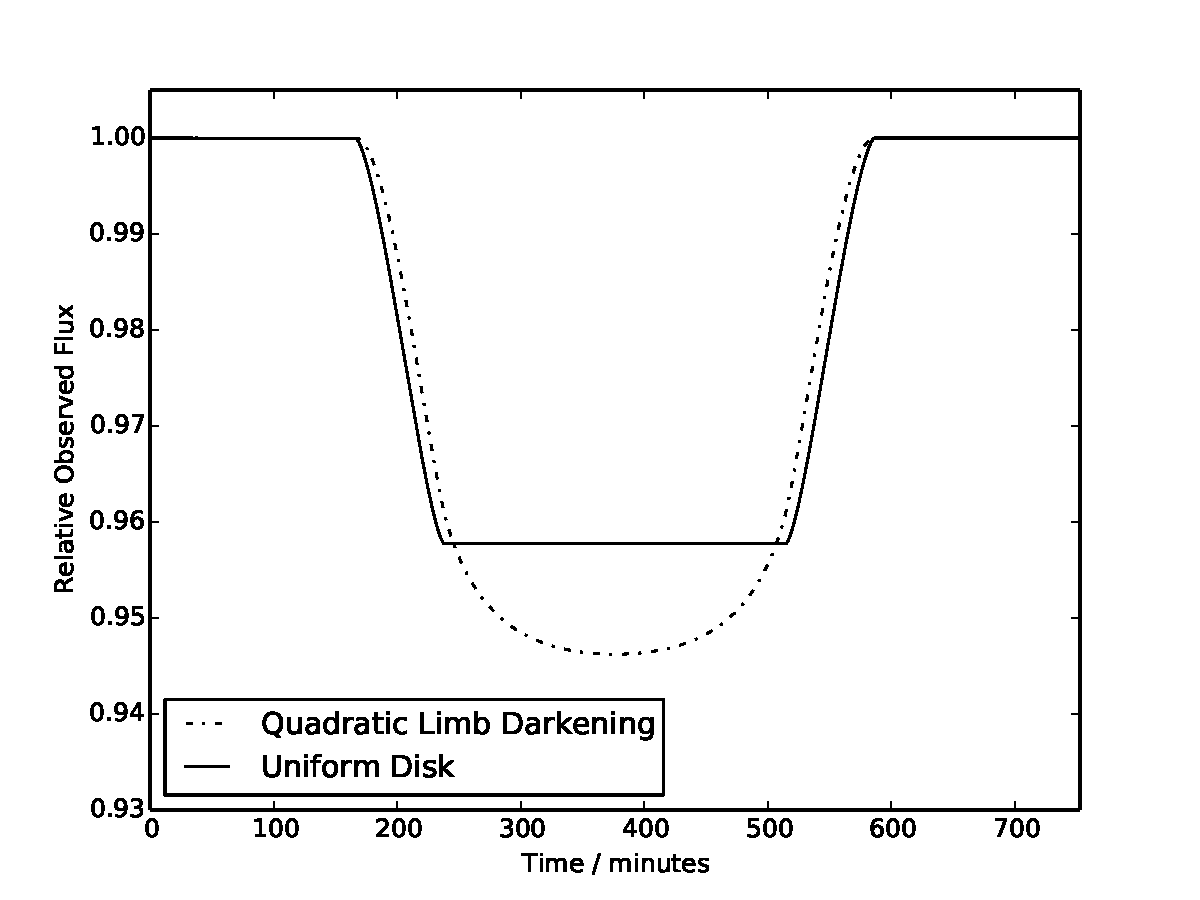
\includegraphics[width=0.7\textwidth]{images/model_comparison.pdf}
    \end{center}
  \end{frame}
  \begin{frame}
  \frametitle{Star Finder}
  SExtractor commonly used, great for well aligned images, but poor when you have multiple frames with various tracking issues and seeing conditions.

  Developed a simple easily modifiable algorithm for source discovery and tracking.
  \begin{center}
    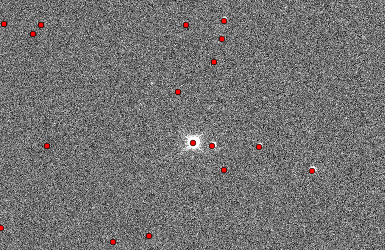
\includegraphics[width=0.7\textwidth]{images/starfinder_zoom.png}
  \end{center}
  \end{frame}
  \begin{frame}
  \frametitle{Star Finder}
    \framesubtitle{Algorithm}
    \begin{itemize}
        \item Estimate a sky background
        \item Filter pixels below some signal to noise to ratio
        \item Find objects greater than a threshold size
        \item Apply a 2D Gaussian to objects to find centers - also gives aperture information
    \end{itemize}
    For subsequent images the Gaussian locater step is repeated to track the stars.
    \begin{center}
        \includegraphics[width=0.3\textwidth]{images/star_untracked.pdf}\quad
        \includegraphics[width=0.3\textwidth]{images/star_tracked.pdf}
    \end{center}
  \end{frame}
\end{document}